\documentclass[12pt, oneside]{article}   	% use "amsart" instead of "article" for AMSLaTeX format
\usepackage{geometry}                		% See geometry.pdf to learn the layout options. There are lots.
\geometry{letterpaper}                   		% ... or a4paper or a5paper or ... 
%\geometry{landscape}                		% Activate for rotated page geometry
%\usepackage[parfill]{parskip}    		% Activate to begin paragraphs with an empty line rather than an indent
\usepackage{graphicx}				% Use pdf, png, jpg, or eps§ with pdflatex; use eps in DVI mode
\graphicspath{ {../figures/} }
								% TeX will automatically convert eps --> pdf in pdflatex		
\usepackage{amssymb}
\usepackage{amsmath}
\usepackage{hyperref}

%SetFonts

%SetFonts


\title{%
	Movie Rating Prediction Using Convolutional Neural Networks}
\author{Christopher Pyles}
\date{March 20, 2020}							% Activate to display a given date or no date

\begin{document}

\maketitle

\section{Introduction}



\section{Data}

The data used in this project is provided by \href{https://api.tmdb.org}{The Movie Database's API (TMDb)}. The data queried covers movies released in 2018 in English, spanning many genres: 

\begin{itemize}
\item Action ($n=245$)
\item Adventure ($n=134$)
\item Animation ($n=117$)
\item Comedy ($n=569$)
\item Crime ($n=155$)
\item Documentary ($n=464$)
\item Drama ($n=764$)
\item Family ($n=148$)
\item Fantasy ($n=144$)
\item History ($n=67$)
\item Horror ($n=446$)
\item Music ($n=126$)
\item Mystery ($n=144$)
\item Romance ($n=222$)
\item Science Fiction ($n=188$)
\item TV Movie ($n=197$)
\item Thriller ($n=511$)
\item War ($n=29$)
\item Western ($n=31$)
\end{itemize}

The data, after being queried, were joined into a single table and written to a CSV file. The columns of interest are described in Table \ref{table:cols_of_interest}. After dropping rows with missing values in the columns of interest, the data contained $n=2700$ rows.

\begin{table}
\begin{center}\begin{tabular}{c|l}
\textbf{Column} & \textbf{Description} \\ \hline
\texttt{id} & \textbf{primary key}, a unique ID number for each movie \\
\texttt{adult} & whether or not the movie is R+ rated \\
\texttt{genre\_ids} & list of genre ID numbers corresponding to \texttt{genres} table \\
\texttt{original\_language} & the language that the movie was originally released in \\
\texttt{original\_title} & the title of the movie \\
\texttt{overview} & movie synopsis \\
\texttt{release\_date} & the date of first release \\
\texttt{vote\_average} & average of rating votes on a 10-point scale \\
\texttt{vote\_count} & the number of votes \\
\texttt{poster\_path} & URL path to movie poster \\
\end{tabular}\end{center}
\caption{\label{table:cols_of_interest}Column descriptions for TMDb API data (the \texttt{movies} table).}
\end{table}

\subsection{Data Cleaning}

Cleaning the data for this project, after dropping missing values, involved rounding the \texttt{vote\_average} column, cleaning the synopsis strings, joining the \texttt{genres} and \texttt{movies} tables, and converting the movie posters into 140 $\times$ 92 $\times$ 3 arrays of RGB values.

The \texttt{vote\_average} column ($\mu = 6.628$, $\sigma = 1.939$) describes the variable of interest, representing the average rating across votes for a single movie. In this analysis, this column will be transformed from a continuous variable into an ordinal variable with possible values 1 to 10 by rounding the vote average to a whole number. After rounding, the distribution of ratings is provided in Figure \ref{fig:rating_barplot}.

\begin{figure}
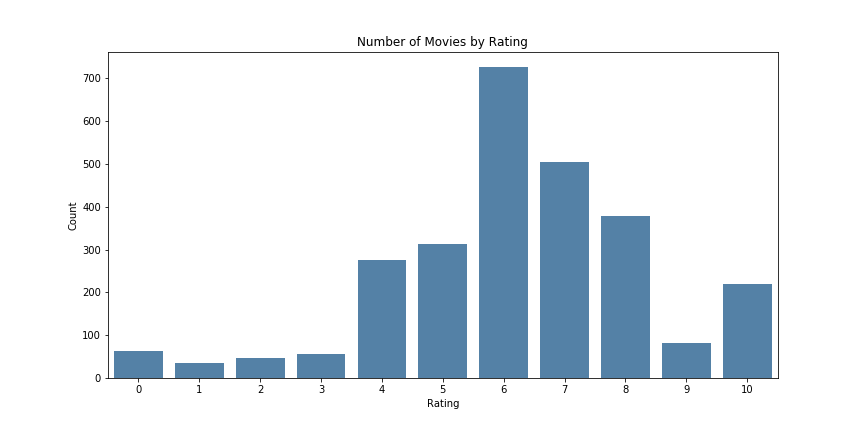
\includegraphics[width=\textwidth]{rating_barplot}
\caption{\label{fig:rating_barplot}Number of movies for each value of ratings, rounded from \texttt{vote\_average}.}
\end{figure}

To clean the movie synopses, all letters were transformed to lowercas, and any characters not matching the regex \texttt{[A-Za-z0-9 ]} were replaced with spaces.

The \texttt{genre\_ids} column is a list of genre IDs encoded as a string, so to start any empty lists, \texttt{"[]"}, were replaced with \texttt{NaN}. Then, the string were split into Python lists of IDs, and were joined with the \texttt{genres} table, so that \texttt{movies} had a column \texttt{genres} where each value is a list of genres for that movie. Figure \ref{fig:genre_barplot} shows the breakdown of movies by genre.

\begin{figure}
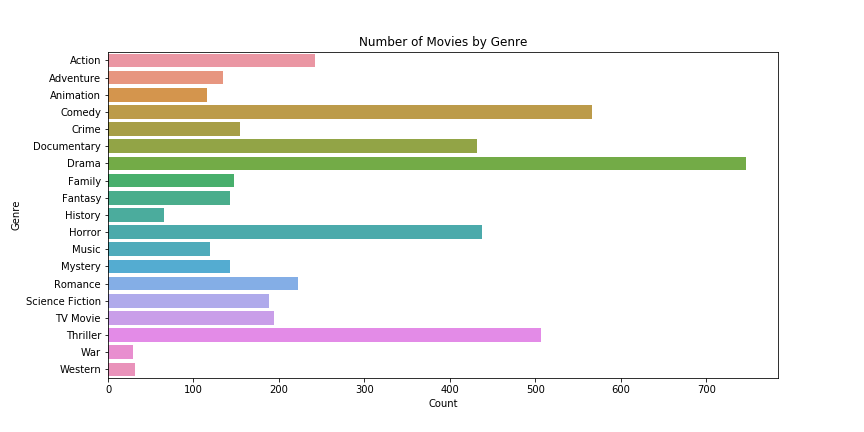
\includegraphics[width=\textwidth]{genre_barplot}
\caption{\label{fig:genre_barplot}Number of movies in each genre.}
\end{figure}

Lastly, each movie poster was downloaded from TMDb and stored as a 140 $\times$ 92 $\times$ 3 array in NumPy, stored as a .mat file. The structure of this file is analagous to a dictionary, where each key is a movie ID (as a string) and each value is the 3-D array of RGB values describing the poster.

\subsection{Exploratory Data Analysis}

Before modeling, a cursory analysis of the data yielded the interesting relationships:

\begin{itemize}

\item Figure \ref{fig:vote_count_by_rating} shows that vote count tends to increase logarithmically with rating until 8, after which it drops significantly. This demonstrates that having more votes tends to "bring down the curve."

\begin{figure}
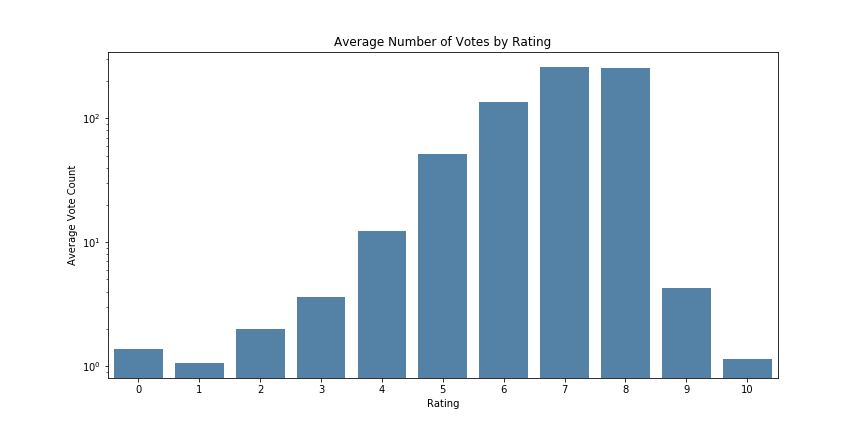
\includegraphics[width=\textwidth]{vote_count_by_rating}
\caption{\label{fig:vote_count_by_rating}Average vote count by rating.}
\end{figure}

\item There are significantly more non-adult movies than adult movies, as demonstrated in Figure \ref{fig:ratings_by_adult}. It is interesting to note that adult movies have a double-peak distribution with far less spread than do the non-adult movies.

\begin{figure}
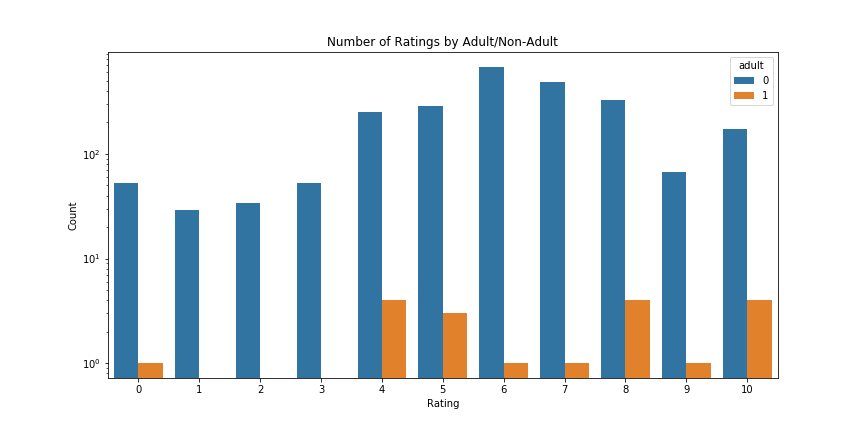
\includegraphics[width=\textwidth]{ratings_by_adult}
\caption{\label{fig:ratings_by_adult}Number of ratings by adult/non-adult.}
\end{figure}

\item Figure \ref{fig:ratings_by_genre} shows the distribution of ratings for each genre.

\begin{figure}
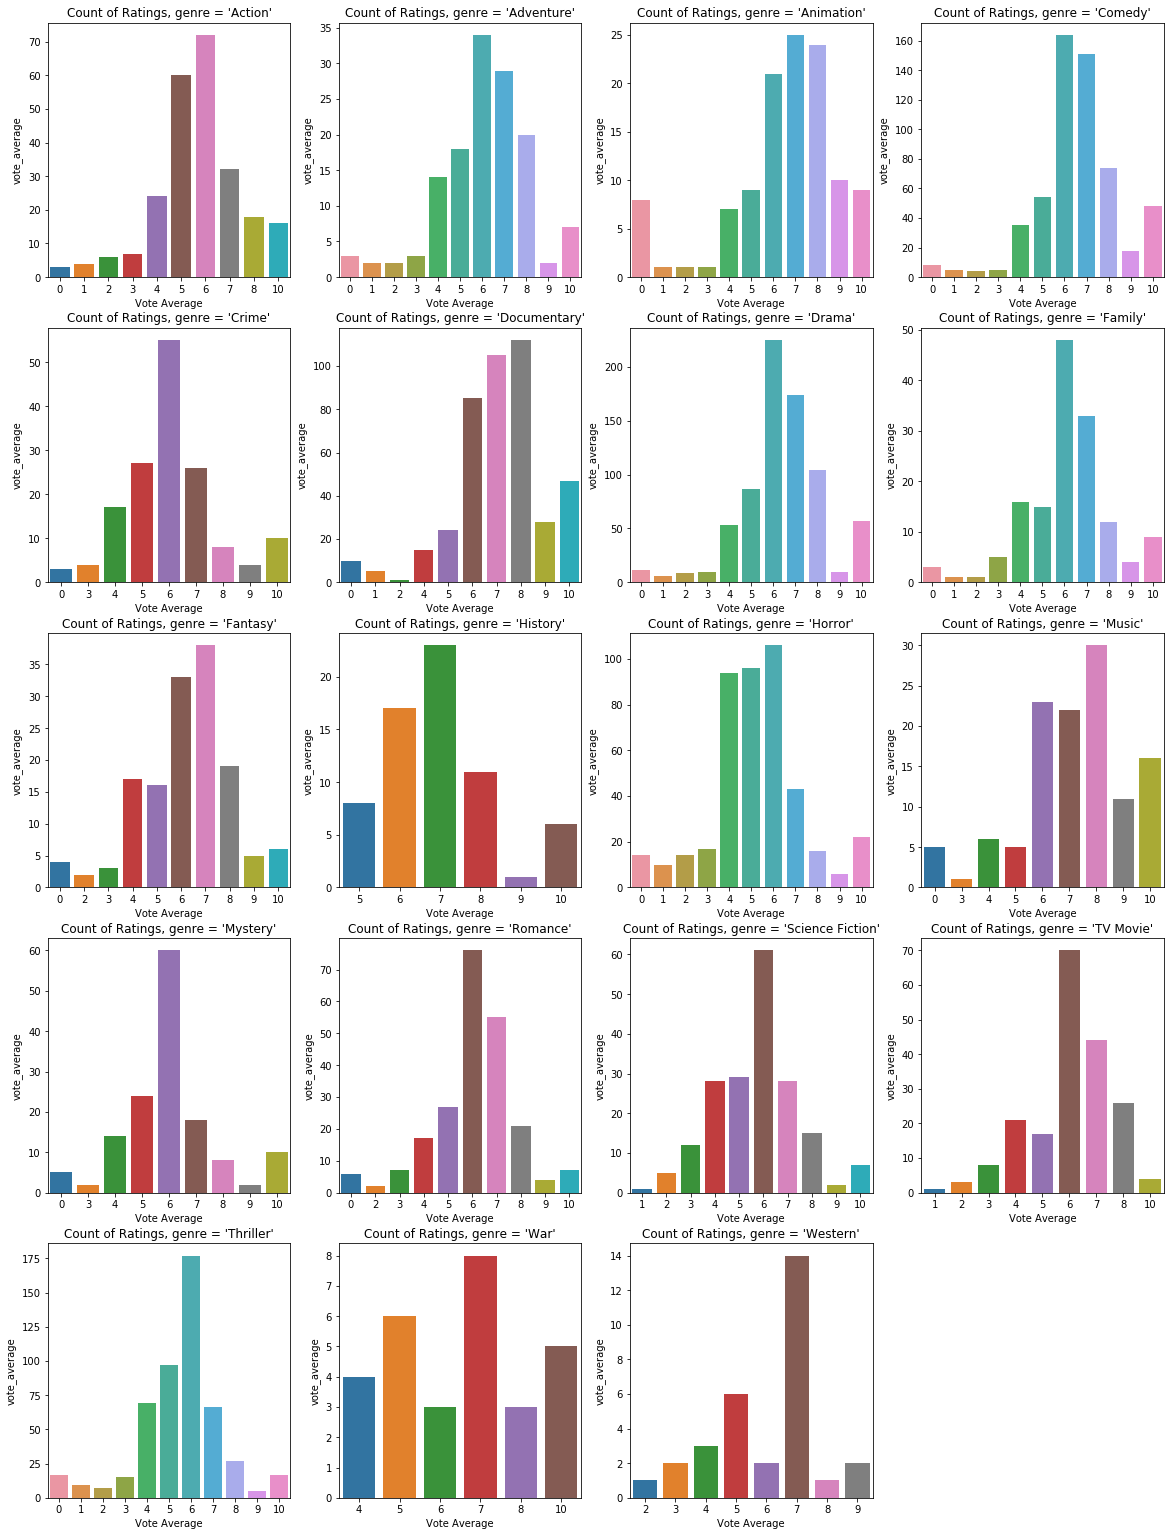
\includegraphics[height=0.9\textheight]{ratings_by_genre}
\caption{\label{fig:ratings_by_genre}Distribution of ratings by genre.}
\end{figure}

\item No discernible relationship is seen between the length of the overview and the movie's rating.

\item The distributions of ratings by release date day of week appear to be different in skew (Figure \ref{fig:ratings_dow}), indicating that this may be an important feature. No discernible relationship is seen between rating and day of month or month of release.

\begin{figure}
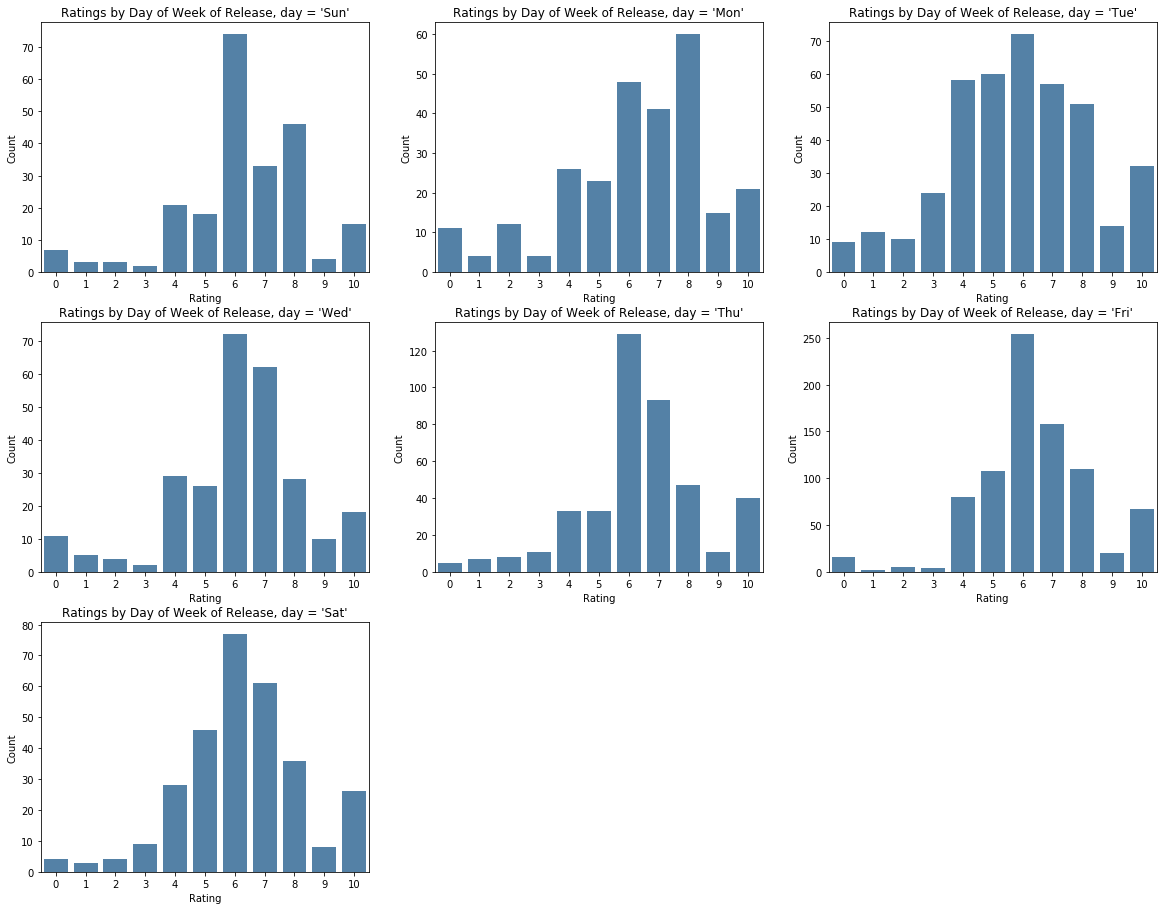
\includegraphics[width=\textwidth]{ratings_dow}
\caption{\label{fig:ratings_dow}Distribution of ratings by day of week of release.}
\end{figure}

\end{itemize}

\section{Analysis}

\subsection{Words in Synopses}

As the first part of this analysis, the statistical significance of the presence of different words in synopses is studied using hypothesis testing. The null hypothesis for this test is that the presence of a word does not affect the average rating, and the alternative is that the presence of the word results in an increase in rating. The test statistic used here is the aboslute difference between the mean rating of movies where the word is present in the synopsis and the movies where it is not. Under the null hypothesis, the truth value of a word being present in a synopsis is shuffled for each observation, so that same number of ``present''s is obtained. Then, the test statistic is computed and the p-value is calculated as the proportion of the test statistic values that are greater than or equal to the observed value for that word.

\subsection{Classification without Posters}

The next step in the analysis is to attempt classification using the features in \texttt{movies} alone (i.e. without the posters). 

\section{Results}

\subsection{Words in Synopses}

\end{document}